\documentclass[11pt]{scrartcl}
\usepackage[utf8]{inputenc} % Kodierung der Textdatei mit Sonderzeichen
\usepackage[ngerman]{babel} % Sprache fuer Inhaltsverzeichnis etc.
\usepackage{amssymb} % Mathematische Symbole
\usepackage{amsmath} % Mehr mathematische Konstrukte
\usepackage{graphicx} % Um Bilder einbinden zu koennen
\usepackage{float} % fuer \begin{figure}[H]
\usepackage{icomma} % laesst das Komma als Dezimaltrennzeichen interpretieren
\usepackage[pdftex]{hyperref} % Hyperlinks im Dokument
\hypersetup{colorlinks=true, linkcolor=black, citecolor=black, filecolor=black, urlcolor=black, pdftitle={Grätzelzelle - Projektpraktikum 09/10 Gruppe 5}}


\newcommand{\unit}[1]{\ensuremath{\,\mathrm{#1}}} % Einheiten schreiben sich immer aufrecht!
\newcommand{\degr}{\ensuremath{^\circ}}
\newcommand{\cel}{\ensuremath{\degr\mathrm{C}}}
\newcommand{\dif}{\ensuremath{\mathrm{d}}}
\newcommand{\pdif}[2]{\ensuremath{\frac{\partial#1}{\partial#2}}}
\newcommand{\ee}[1]{\ensuremath{\cdot 10^{#1}}}


\setlength{\parindent}{0pt}
\setlength{\parskip}{0.5\baselineskip}


\title{Gr\"atzelzelle - Gruppe 5 WS 09/10, Projektpraktikum der Uni Erlangen}
\date{19.10.2009 -- 31.10.2009}
\author{Michele Collodo, Andreas Glossner, Karl-Christoph G\"odel, Bastian Hacker, Maria Obst, Alexander Wagner, David Winnekens}



\begin{document}
\sloppy % laesst Latex nicht ueber den Rand rausschreiben
\thispagestyle{empty}
\large{Projektpraktikum WS 09/10}
\hfill
\raisebox{-1.4cm}{
\includegraphics[width=5cm]{images/fau.pdf}}
\\[8\baselineskip]
\begin{center}
{\Huge\textbf{Gr\"atzelzelle}}
\\[0.5\baselineskip]
{\large Energieforschung auf der Nanoebene}
\\[1.5\baselineskip]
{\Large 19.10.2009 -- 31.10.2009}
\\[6\baselineskip]
{\huge\textbf{PPG 5}}\\[0.5\baselineskip]
{\large\textbf{
Michele Collodo,
Andreas Glossner,\\
Karl-Christoph G\"odel,
Bastian Hacker,\\
Maria Obst,
Alexander Wagner,
David Winnekens}\\
Tutor: Xiaoyue Jin}
\vfill



\small{\url{http://pp.physik.uni-erlangen.de/groups/ws0910/ppg5/ppg5\_start.html}}
\end{center}
\newpage



\tableofcontents
\vfill



\begin{abstract}
Ziel dieses Projekts war es, eine funktionierende Grätzelzelle -- eine alternative Form von Solarzellen -- herzustellen und deren Eigenschaften zu untersuchen.

Unter Bestrahlung der Zelle mit einer hellen LED und Zwischenschaltung verschieden gro\ss{}er Widerst\"ande konnte eine elektrische Leistung von bis zu $284\unit{nW}$ erzeugt werden, was einem Wirkungsgrad von knapp $1\unit{ppm}$ entspricht. Eine andere, mit rotem Farbstoff versehene Zelle, zeigte im Licht kurzwelliger LEDs eine deutlich h\"ohere Empfindlichkeit als bei langwelligen LEDs.

\end{abstract}
\newpage





\section{Einleitung}

% Ist das zu viel Blabla?
Ein großes Problem der an sich viel versprechenden Solartechnik bleiben nach wie vor die enormen Kosten im Vergleich zur Energieerzeugung mit fossilen Brennstoffen. Die in den neunziger Jahren von Michael Grätzel von der EPFL Lausanne entwickelte und seitdem stetig verbesserte Farbstoff\-solarzelle ("`Grätzelzelle"') ermöglicht im Vergleich zu herkömmlichen, siliziumbasierten Solarzellen die Möglichkeit einer relativ kostengünstigen Herstellung und könnte deswegen in Zukunft mit zur Lösung der Energieproblematik beitragen. Nicht zuletzt auf Grund dessen, aber auch weil eine solche Zelle leicht herzustellen ist, waren die nachfolgend beschriebenen Untersuchungen an der Grätzelzelle Thema des ersten Projektpraktikumsversuchs.\ldots





\section{Theorie}
\subsection{B\"andermodell und Halbleitertechnik}
Um die Funktionsweise von Solarzellen im allgemeinen und der Gr\"atzelzelle im besonderen verstehen zu k\"onnen, muss man sich zun\"achst mit dem Energieb\"andermodell aus der Quantenmechanik besch\"aftigen. Die B\"ander entstehen durch \"Uberlagerung der Energieniveaus der einzelnen, im Kristall dicht nebeneinander gelagerten Atome. Nahe bei den Atomr\"umpfen befinden sich die gebundenen Zust\"ande. Wenig dar\"uber entsteht durch \"Uberlappung der Potentiale das Valenzband, in dem alle Pl\"atze mit Elektronen besetzt sind. So kann sich ein Elektron nur bewegen, wenn sich ein anderes Elektron genau in entgegengesetzter Richtung bewegt. 
Noch weiter von den Atomr\"umpfen entfernt liegen weitere, unbesetzte Energieniveaus \"ubereinander. Hier k\"onnen sich die Elektronen frei bewegen, dieses Band wird daher Leitungsband genannt.

Zwischen Valenz- und Leitungsband befindet sich die verbotene Zone (Bandl\"ucke), in der sich keine Elektronen befinden. Nach der Gr\"o\ss{}e dieser Zone unterscheidet man Leiter, Halbleiter und Isolatoren. Bei einem Leiter gibt es keine verbotene Zone und Valenz- und Leitungsband gehen ineinander \"uber oder im Valenzband sind nicht alle Pl\"atze mit Elektronen besetzt. So kann problemlos Strom fließen. Isolatoren hingegen haben ein vollst\"andig besetztes Valenzband und die Bandl\"ucke ist so gro\ss{}, dass sie selbst von hoch angeregten Elektronen nicht oder nur sehr schwer \"uberwunden werden kann.

Auch bei Halbleitern ist das Valenzband voll besetzt, jedoch ist hier die verbotene Zone noch kleiner als etwa $10\unit{eV}$. Es ist also f\"ur Elektronen, die durch hohe Temperaturen oder einfallende Photonen angeregt sind, m\"oglich, die L\"ucke zu \"uberspringen und sich im Leitungsband fortzubewegen. Werden hier nun in den Kristall Fremdatome eingef\"ugt (Dotierung), ver\"andern sich dessen leitenden Eigenschaften. Werden Atome eingesetzt, die mehr Elektronen in der \"au\ss{}eren Schale haben als die des Kristalls (n-Dotierung), so gibt es \glqq\"ubersch\"ussige\grqq{} Elektronen, die einfacher ins Leitungsband wechseln k\"onnen. Solche Atome hei\ss{}en Elektronendonatoren. F\"ugt man hingegen Fremdatome ein, die weniger Elektronen in ihrer \"au\ss{}eren Schale haben (p-Dotierung), entstehen L\"ocher, in denen leicht Elektronen aus dem Valenzband angelagert werden. Es gibt nun Elektronenfehlstellen, die Atome werden als Elektronenakzeptoren bezeichnet.

Bringt man nun einen p-dotierten und einen n-dotierten Halbleiter zusammen, diffundieren die \"ubersch\"ussigen Elektronen aus der n-Schicht zu den Fehlstellen in der p-Schicht, es bildet sich ein elektrisches Feld, das von der n- zur p-Seite gerichtet ist. Nun k\"onnen durch das Anlegen einer \"au\ss{}eren Spannung verschiedene Funktionen, wie beispielsweise die Diode, erreicht werden. Schließt man den Pluspol an die p-Schicht und den Minuspol an die n-Schicht, betreibt man eine Diode in Durchlassrichtung. Die Bandl\"ucke wird beinahe aufgehoben und Leitung ist m\"oglich.

Bei umgekehrter Polung, also in Sperrrichtung, kann kein Strom flie\ss{}en. Solche Dioden nennt man Photodioden, sie werden in herk\"ommlichen Solarzellen verwendet. Eine Gr\"atzelzelle hingegen greift mehr auf Ideen der Natur zur\"uck. Hier wird durch Imitation der nat\"urlichen Photosynthese Energie erzeugt.



\subsection{Funktionsweise der Gr\"atzelzelle}
Die Gr\"atzelzelle, benannt nach ihrem Erfinder, dem Schweizer Michael Gr\"atzel, besteht aus zwei Elektroden, typischerweise leitend beschichteten Glasplatten. Auf der einen Glasplatte wird als Halbleiter Titandioxid angebracht. Da hier aber die verbotene Zone aber eine Gr\"o\ss{}e von $3.2\unit{eV}$ hat, w\"are die Zelle nur f\"ur hoch-energetische Photonen des UV-Lichts empfindlich. Daher wird auf die TiO$_{2}$-Schicht ein lichtempfindlicher organischer Farbstoff aufgebracht, dessen Elektronen auch von sichtbarem Licht angeregt werden k\"onnen. Die Gr\"atzelzelle wird deshalb auch als Farbstoffsolarzelle bezeichnet.

Die Gegenelektrode ist mit einem Katalysator, oft Platin, beschichtet, um die \"Ubergabe der ausgel\"osten Elektronen zu erleichtern. Den Raum zwischen den beiden Elektroden f\"ullt ein Elektrolyt, der in Redox-Reaktionen einerseits dem Farbstoff schnellen Nachschub an Elektronen liefert und andererseits an der Kathode wieder zur\"uck reagiert. Hier wird h\"aufig Iodkaliumiodid eingesetzt.





\section{Aufbau}
\subsection{Materialien, Beschaffung und Bau der Zelle}
%%% Karl
Die Beschaffung der f\"ur den Bau ben\"otigten Materialien stellte zu Beginn ein Problem dar. Insbesondere war es schwer, leitende und gleichzeitig transparente Elektroden zu bekommen. Die erste M\"oglichkeit, mit Gold beschichtet Glaspl\"attchen, zu verwenden, scheiterte an den zu geringen Ausma\ss{}en der m\"oglichen Tr\"agerplatten. Zu lange Lieferzeiten und zu hohe Preise schlossen auch die Bestellung von industriell produzierten ITO-Gl\"asern (Indiumzinnoxid-Beschichtung) aus.

\begin{figure}[ht]
\begin{center}
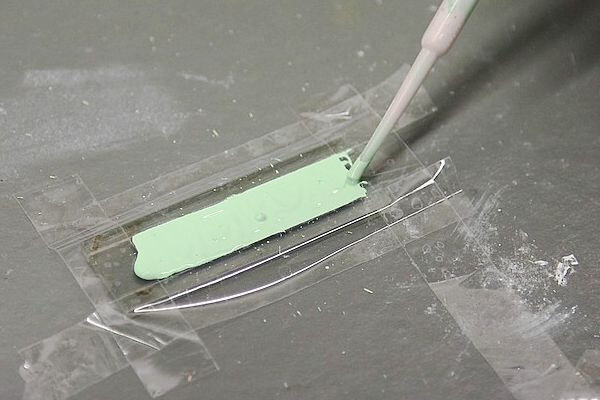
\includegraphics[width=0.8\textwidth]{images/herstellung_pipette.jpg}
\end{center}
\vspace{-1.5\baselineskip}
\caption{Aufbringen der eingefärbten Titandioxid Paste}
\label{herstellung_pipette}
\end{figure}

Das Institut der Physikalischen Chemie der Universit\"at Erlangen stellte gl\"ucklicherweise mehrere Fluorzinnoxid (FTO) beschichtete Glasplatten zur Verf\"ugung. Die leitend beschichteten, transparenten Glasplatten waren bereits auf eine Gr\"o\ss{}e von \(70\unit{mm} \times 20\unit{mm} \times 4 \unit{mm}\) zugeschnitten. Auf der leitenden Seite der Glasplatte konnte mit Hilfe eines Multimeters ein Widerstand von etwa \(20 \unit{\frac{\Omega}{cm}}\) gemessen werden.

Das Elektrolyt, eine Iod-Kaliumiodid-L\"osung sowie verd\"unnte Salzs\"aure zum Anmischen der Titandioxidpaste konnten ebenfalls von der Physikalischen Chemie bezogen werden.

\begin{figure}[ht]
\begin{center}
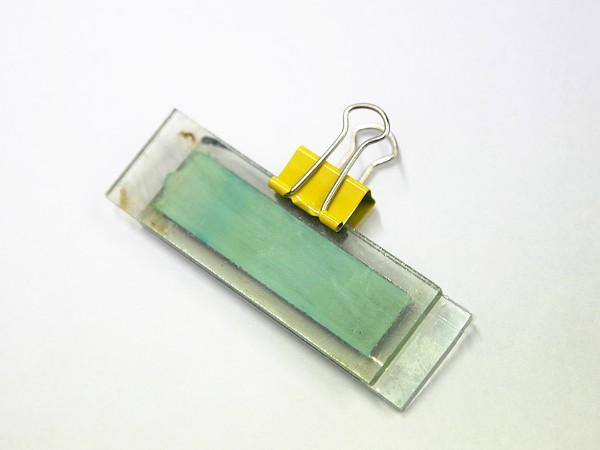
\includegraphics[width=0.8\textwidth]{images/zelle_gruen.jpg}
\end{center}
\vspace{-1.5\baselineskip}
\caption{Die fertige Zelle}
\label{zelle_gruen.jpg}
\end{figure}



\subsection{Versuchsanordnung} %%% Michele und Axi
%%% noch weiter untergliedern? vorueberlegung, LED, Wellenlaenge, Leistung? -> nein
Das erste Ziel war die Bestimmung der Abh\"angigkeit der Leistung der Zelle von der Wellenl\"ange des eingestrahlten Lichts. Zun\"achst wollten wir dieses Spektrum mit einem Gitter erzeugen. Die ersten Versuche mit einem Aufbau aus Baustrahler, Linse und Gitter auf einer optischen Bank hatten jedoch bereits gezeigt, dass die zu erwartende Lichtst\"arke des aufgef\"acherten Spektrums viel zu schwach f\"ur eine Messung sein w\"urde. Außerdem wurden die einzelnen Linien des Spektrums viel zu schwach aufgef\"achert, so dass nicht nur ein Farbbereich auf die breitere Zelle treffen w\"urde. Auch der Ersatz des Gitters durch ein Prisma konnte diese Probleme nicht l\"osen.

Deshalb haben wir uns entschlossen, die verschiedenen Farbbereiche durch LEDs unterschiedlicher Wellenl\"ange darzustellen. Hierbei kam ein Verbund aus zehn verschiedenen LEDs des Modells Luxeon K2 von Philips\footnote{\url{http://www.led-tech.de/produkt-pdf/luxeon/DS51\_Luxeon\_K2.pdf}} zum Einsatz, welcher bereits fr\"uher von einem Gruppenmitglied gebaut wurde.

Es wurden 3 weiße sowie 7 farbige LEDs verwendet (Tabelle \ref{leds}), wobei die roten bis amberfarbenen LEDs mit $700 \unit{mA}$, die restlichen mit $1000 \unit{mA}$ bestromt wurden. Die LEDs sind einzeln dimmbar, sie wurden jedoch stets bei maximaler Leuchtst\"arke betrieben. Um den Abstrahlwinkel von $140\degr$ einzuschränken kam zusätzlich eine Linse\footnote{Datenblatt: \url{http://www.farnell.com/datasheets/16887.pdf}} mit einer FWHM von $10\degr$ zum Einsatz.

\begin{table}[ht]
\captionabove{Daten der verwendeten LEDs}
\label{leds}
\begin{center}\vspace{-\baselineskip}
\begin{tabular}{l|cccc}
&Farbe &
$\lambda_{\text{Peak}} \unit{[nm]}$ &
FWHM $\unit{[nm]}$ &
typ. Lichtstrom $\unit{[lm]}$ (Bin)\\
\hline
LED1 & rot		& $627 \pm 18$		& 20	& 75 (R)	\\
LED2 & orange		& $617 \pm 3,5$		& 20	& 100 (S)	\\
LED3 & amber		& $590 \pm 7$		& 14	& 75 (R)	\\
LED4 & grün		& $530 \pm 20$		& 35	& 100 (U)	\\
LED5 & cyan		& $505 \pm 15$		& 30	& 80 (T)	\\
LED6 & blau		& $470 \pm 20$		& 25	& 27 (P)	\\
LED7 & royal-blau	& $455 \pm 15$		& 20	& $475 \unit{mW}$ (Q)\\
LED8 & kalt-weiß	& $6500\pm 3500\unit{K}$& n/a	& 120 (V)	\\
LED9 & neutral-weiß	& $4100\pm 600 \unit{K}$& n/a	& 120 (V)	\\
LED10 & warm-weiß	& $3000\pm 500 \unit{K}$& n/a	& 100 (U)	
\end{tabular}
\vspace{-\baselineskip}\end{center}
\end{table}


Um eine Vergleichsmessung wie die Wellenl\"angenabh\"angigkeit genau durchf\"uhren zu k\"onnen, muss der Aufbau bei jeder Einzelmessung genau gleich sein. Daf\"ur wurde die Gr\"atzelzelle in eine Halterung aus Klemmen und Stativstangen eingespannt. Der Verbund aus LEDs wurde entlang der Grundplatte des Aufbaus unter die Zelle geschoben. Zwischen LED und Zelle kam eine Blende mit \"Offnungsdurchmesser $1,8\unit{cm}$ zum Einsatz, um in etwa den Teil des Lichtkegels zu nutzen, der auch vom Luxsensor empfangen wird. Eine weitere Stativstange markierte dabei die Stelle, an der sich die momentan verwendete LED befinden musste, um jeweils genau senkrecht unter Zelle positioniert zu sein. Der vertikale Abstand LED - Zelle betrug dabei ca. $12\unit{cm}$.

\begin{figure}[ht]
\begin{center}
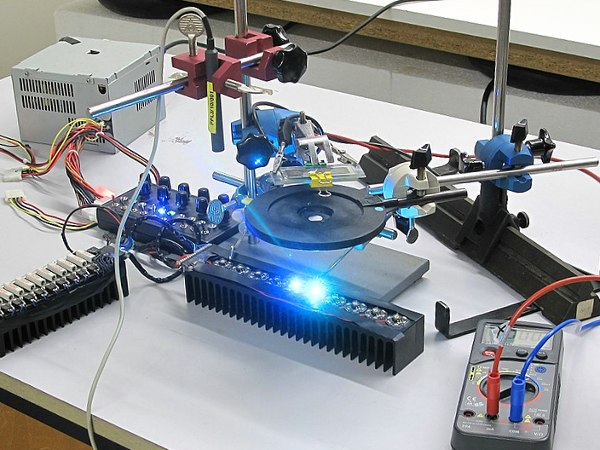
\includegraphics[width=1.0\textwidth]{images/messung_farben.jpg}
\end{center}
\vspace{-1.5\baselineskip}
\caption{Aufbau zur Messung der Wellenlängenabhängigkeit. Der Luxsensor ist die graue vertikale Sonde. Die Zelle befindet sich über der Blende.}
\label{messung_farben}
\end{figure}

In der selben H\"ohe wurde, versetzt zur Zelle, auch ein LUX-Sensor befestigt, um eine Messung der jeweiligen Leuchtkraft der LEDs zu erm\"oglichen. Auch hier markierte eine Stativstange die Messposition. Zum Auslesen des Sensor wurde das CASSY-LAB verwendet, welches die Messwerte \"uber $1000\unit{ms}$ gemittelt anzeigte.

Die Messung, der von der Zelle gelieferten Spannung, erfolgte zum Einen durch ein direkt an die Zelle angeschlossenes Multimeter, sowie durch ein weiteres Multimeter, dessen Signal jedoch zun\"achst einen Messverst\"arker durchlief. Der genau Aufbau ist auch aus dem folgenden Schaltplan sowie dem Foto ersichtlich.

%hier fehlt Schaltplan + Foto

Bei der Messung wurde jeweils zwei Minuten gewartet, bis sich die Messwerte eingependelt hatten.
%%% gehoert das hier hin? eigentlich nein, oder?

Der zweite Teil der Messung umfasste die Bestimmung der Leistung der Solarzelle in verschiedenen Widerstandsbereichen. Hierbei wurde nur die LED Nr.~7 (Farbe~blau) verwendet, da sie die h\"ochsten Spannungen geliefert hat. Au\ss{}erdem kam eine neue Gr\"atzelzelle zum Einsatz, da die Zelle der ersten Messung bereits eingetrocknet war.

Der Aufbau der LEDs wurde leicht angepasst. Neben einem geringeren Abstand der Lichtquelle von der Zelle, ersetzte eine Linse die Lochblende zum Fokussieren des Lichtstrahls. (Abb. \ref{messung_leistung})

Die Messung der Strom- und Spannungswerte wurde mit einem Multimeter f\"ur die Spannung und einem Amperemeter f\"ur die Stromst\"arke durchgef\"uhrt. Der Einsatz eines Messverst\"arkers war hierbei nicht m\"oglich, da die anschlie\ss{}end am Multimeter abzulesenden Werte sehr starke Schwankungen aufwie\ss{}en und einen willkürlichen Offset enthielten.

\begin{figure}[ht]
\begin{center}
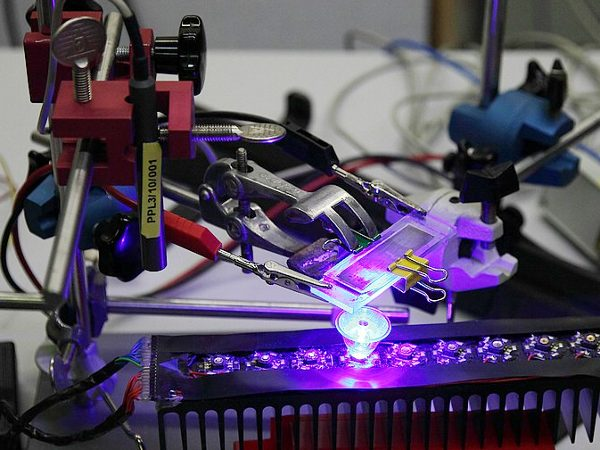
\includegraphics[width=0.8\textwidth]{images/messung_leistung.jpg}
\end{center}
\vspace{-1.5\baselineskip}
\caption{Aufbau zur Messung der Leistung}
\label{messung_leistung}
\end{figure}

Der Aufbau sowie die verwendeten Bauteile sind wiederum im Schaltplan (Abb.~\ref{leistungsschaltkreis}) sowie dem ?Foto? illustriert.

\begin{figure}[ht]
\begin{center}
%%% Zeichnung mit xcircuit
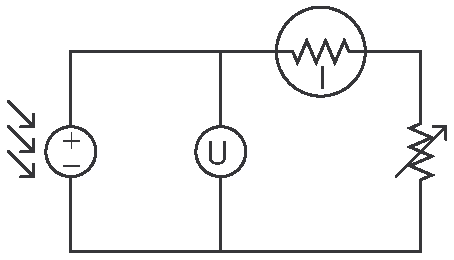
\includegraphics[width=0.8\textwidth]{images/leistungsmesskreis.pdf}
\end{center}
\vspace{-1.5\baselineskip}
\caption{Schaltkreis zur Leistungsmessung. Das Amperemeter hatte einen signifikanten Eigenwiderstand.}
\label{leistungsschaltkreis}
\end{figure}

Um mehrere Paare an Messwerten zu erhalten, wurde wie zu sehen ist, ein regelbarer Widerstand zwischengeschaltet und die Messung mit verschiedenen Kombinationen der Widerst\"ande durchgef\"uhrt. Leider hatte auch das Amperemeter einen Eigenwiderstand. Dieser hat allerdings die Messmethode nicht nachhaltig beeinflusst. ($\rightarrow$ vgl. Ergebnisse) %%% gehoert das hier hin?





\section{Messungen und Ergebnisse}
%%% Basti, Michele (LED's)
\subsection{Leistung und Wirkungsgrad}
Zur Leistungsmessung wurden die Strom- und Spannungswerte der Zelle mit einer spannungsrichtigen Schaltung nach (Abb.~\ref{leistungsschaltkreis}) bei verschiedenen Lastwiderständen gemessen. Die Lastwiderstände waren über eine Kombinationsbox einstell- und ablesbar. Das Voltmeter hatte mit $10\unit{M\Omega}$ genügend Eigenwiderstand, um die Messung nicht zu beeinflussen. Das Amperemeter hatte jedoch wegen der hohen benötigten Empfindlichkeit einen signifikanten Eigenwiderstand von
\[
R_I = 5,22\pm 0,03 \unit{k\Omega}
\qquad\qquad\qquad
R = R_I+R_{\text{L}}\;.
\]
Der zusätzliche Lastwiderstand $R_{\text{L}}$ wurde nun im Bereich 0 -- $40\unit{k\Omega}$ variiert und es wurden jeweils wenige Minuten gewartet bis sich stationäre Werte einstellten. Die Messwerte sind in Tabelle \ref{leistungsmesstabelle} angegeben.
\begin{table}[ht]
\captionabove{Messwerte zur Leistungsbestimmung}
\label{leistungsmesstabelle}
\begin{center}\vspace{-\baselineskip}
\begin{tabular}{rr|ccc}
$R_{\text{L}}\; \unit{[k\Omega]}$ &
$R\; \unit{[k\Omega]}$ &
$U\; \unit{[mV]}$ &
$I\; \unit{[\mu A]}$ &
$P\; \unit{[nW]}$ \\
\hline
0	& 5,2	& 34,5	& 6,2	& 214 \\
1	& 6,2	& 38,0	& 5,9	& 224 \\
5	& 10,2	& 52,4	& 5,1	& 267 \\
10	& 15,2	& 66,0	& 4,3	& 284 \\
15	& 20,2	& 75,1	& 3,7	& 278 \\
20	& 25,2	& 82,3	& 3,2	& 263 \\
25	& 30,2	& 88,8	& 2,9	& 258 \\
30	& 35,2	& 93,3	& 2,6	& 243 \\
35	& 40,2	& 96,5	& 2,4	& 232 \\
40	& 45,2	& 99,7	& 2,3	& 229
\end{tabular}
\vspace{-\baselineskip}\end{center}
\end{table}
Die Ableseungenauigkeit durch die begrenzte Anzeigegenauigkeit und Messwertschwankungen betrugen:
\[
\Delta R_{\text{L}} = 1\% R
\qquad\quad
\Delta U = 1\unit{mV}
\qquad\quad
\Delta I = 0,2\unit{\mu A}
\]
Die größte Ungenauigkeit lag also im Messen der winzigen Ströme. Diese haben sowohl einen Einzelfehler als auch einen korelierten Offsetfehler von $0,1\unit{\mu A}$, also insgesamt bis zu 6\%.

Der Leistungsverlauf zeigt ein Maximum bei mittleren Widerständen (im Bereich des Eigenwiderstandes der Zelle). Bei geringen Widerständen wird der Großteil der Leistung in der Zelle selbst freigesetzt und bei hohem Widerstand sorgt der geringe Stromfluss für eine schlechte Leistungsausbeute.
\begin{figure}[ht]
\begin{center}
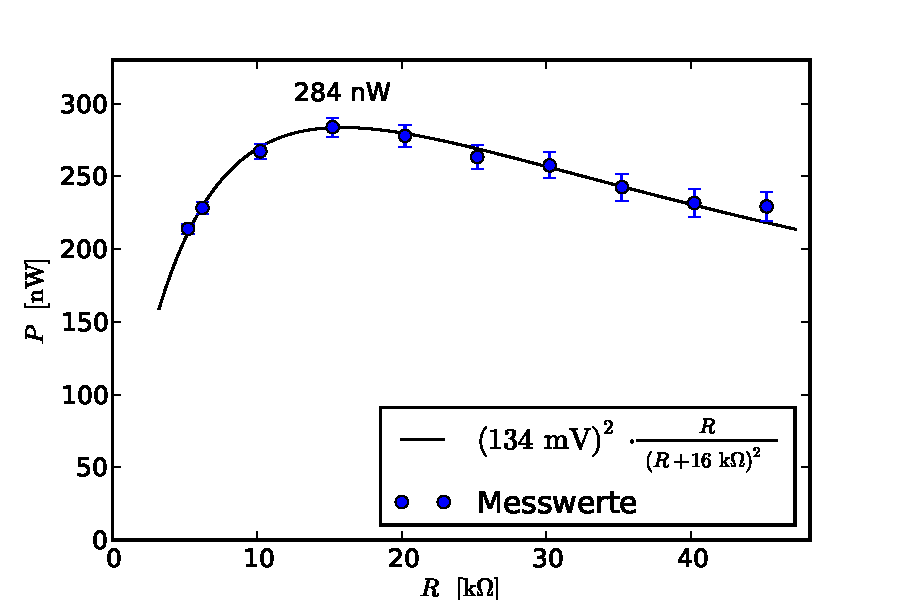
\includegraphics[width=1.0\textwidth]{images/graetzel_leistung.pdf}
\end{center}
\vspace{-1.5\baselineskip}
\caption{Leisungskurve in Abhängigkeit vom äußeren Widerstand. Auf die Daten wurde das Modell einer widerstandsbehafteten Spannungsquelle gefittet.}
\label{leistungskurve}
\end{figure}
Abb. \ref{leistungskurve} zeigt den Verlauf der Leistung zusammen mit dem Modell einer widerstandsbehafteten Spannungsquelle. Der theoretische Leistungsverlauf wäre hier:
\[
P(R)= U_{\text{Last}}\cdot I
= U_{\text{Last}}\cdot \frac{U_{\text{Zelle}}}{R+R_{\text{Zelle}}}
\]
\[
= \left(U_{\text{Zelle}}\cdot \frac{R}{R+R_{\text{Zelle}}}\right)\cdot \frac{U_{\text{Zelle}}}{R+R_{\text{Zelle}}}
= U_{\text{Zelle}}^2\cdot \frac{R}{(R+R_{\text{Zelle}})^2}
\]
Auf die Messdaten wurden nun die Zellspannung $U$ und der Eigenwiderstand $R_{\text{Zelle}}$ gefittet. Die Best-fit Werte sind:
\[
U = 135 \pm 3\unit{mV}
\qquad\qquad
R_{\text{Zelle}} = 16,0 \pm 0,7\unit{k\Omega}
\qquad\qquad
P_{\text{max}} = 284 \pm 4\unit{nW}
\]
Die Spannung erreicht hier einen sehr zufriedenstellenden Wert im $0,1\unit{V}$ Bereich, also in der Größenordnung kommerzieller Zellen. Der Innenwiderstand von ca. $16\unit{k\Omega}$ ist jedoch viel zu groß um eine vernünftige Leistung zu erzeugen. Hierdurch konnte die Zelle im Endeffekt auch nicht wirklich "`unter Last"' getestet werden und die tatsächliche Leistungsfähigkeit von Grätzelzellen entzieht sich unserer Untersuchung.

Die eingestrahlte Leistung in diesem Versuchsteil ermittelt sich aus der verwendeten Leuchtdiode,
diese emittiert unter optimalen Bedingungen eine Leistung von $475 \unit{mW}$\footnote{vgl. \url{http://www.led-tech.de/produkt-pdf/luxeon/DS51\_Luxeon\_K2.pdf}, bei der verwendeten LED handelt es sich um die LXK2 PR14 Q00}, in unserer Anwendung kann der Wert allerdings wegen der erhöhten Chiptemperatur und bereits vorhandener Degradation auf $400 \unit{mW}$ geschätzt werden.
Der Transmissionsgrad der verwendeten Linse\footnote{Fraen FHS-HNB1-LB01-H, Datenblatt siehe \url{http://www.farnell.com/datasheets/16887.pdf}} liegt bei 85\%, der Halbwerts-Öffnungswinkel bei $10\degr$.
Die bestrahlte Fläche der Grätzelzelle beträgt $1,5 \unit{cm} \times 1,5 \unit{cm}$ und befindet sich in einem Abstand vom $5 \unit{cm}$ zur LED, es kann also angenommen werden, dass der gesamte Lichtstrom auf die Zelle gebündelt wird, wodurch sich die eingestrahlte Leistung also zu $340 \unit{mW}$ ergibt.
In Relation zur ermittelten Leistung der Zelle liegt der tatsächlich erreichte Wirkungsgrad also bei
\[
\boxed{\eta = 8 \ee{-7}} \;.
\]

\subsection{Wellenl\"ange}
Zur Ermittlung der Wellenlängenabhängigkeit der Zellleistung wurde eine einfachere Schaltung verwendet, da hier nur die relativen Werte interessant sind. Dieses Mal wurde nicht die erzielte Leistung am Lastwiderstand gemessen, sondern lediglich die direkt an der Zelle abgegriffene Spannung. Eine sinnvolle Stromstärkenmessung stand uns hier noch nicht zur Verfügung, aber da die Spannung weit von einem Sättigungsniveau entfernt war, lassen sich daraus brauchbare Werte für die erzeugte Zellleistung ableiten. Die Spannungswerte lagen mit ca. $2\unit{mV}$ gefährlich nahe am minimal messbaren Signal von $0,1\unit{mV}$, weshalb das Multimetersignal nur zur Kalibration der Mittelwerte verwendet wurde und genauere -- jedoch verschobene -- Werte vom Messverstärker abgelesen wurden. Während der Messung wurde mehrfach die Dunkelspannung ohne Beleuchtung abgelesen, die vom Anfang bis zum Ende der Messung von $U_0=1,9\unit{mV}$ bis $1,6\unit{mV}$ abdriftete. Da uns hier nur das vom Licht erzeugte Signal interessiert, wurde zu jedem Messzeitpunkt der linear interpolierte Dunkelspannungswert subtrahiert. Die Netto-Spannungswerte jeder Leuchtdiode sind in Tabelle \ref{ledspannung} eingetragen. Die grüne Leuchtdiode LED4 wurde aus den Messdaten herausgenommen, weil ihre Leuchtkraft unterhalb des messbaren Bereichs lag.
\begin{table}[ht]
\captionabove{Messwerte zur Wellenlängenabhängigkeit. Die Wellenlängen der Leuchtdioden sind der Herstellerbeschreibung entnommen.}
\label{ledspannung}
\begin{center}\vspace{-\baselineskip}
\begin{tabular}{l|ccc}
\# &
$\lambda\; \unit{[nm]}$ &
$U\; \unit{[mV]}$ &
$E\; \unit{[klux]}$ \\
\hline
LED1	& 627	& 0.258	& 1.79 \\
LED2	& 617	& 0.324	& 1.65 \\
LED3	& 590	& 0.202	& 0.486 \\
LED5	& 505	& 2.738	& 1.698 \\
LED6	& 470	& 5.148	& 1.965 \\
LED7	& 455	& 6.550	& 2.031 \\
\hline
LED8	& 6500\unit{K}	& 4.652	& 2.796 \\
LED9	& 4100\unit{K}	& 2.514	& 2.152 \\
LED10	& 3000\unit{K}	& 2.026	& 2.136
\end{tabular}
\vspace{-\baselineskip}\end{center}
\end{table}


\subsubsection{Ermittlung der LED-Helligkeiten}
Die Wellenlängenabhängigkeit der Photozellenempfindlichkeit kann nur dann ermittelt werden, wenn auch die tatsächlich eingestrahlte Beleuchtungsstärke bekannt ist. Hierzu dient die Vergleichsmessung mit dem Cassy-Luxmeter. Doch auch dieses hat eine eigene Wellenlängenabhängigkeit. Auf der Herstellerseite von Leybold heißt es dazu: "`Der Photometerkopf besteht aus einem Si-Photoelement mit l-Filter zur Anpassung des Photoelements an die spektrale Empfindlichkeit des Auges. Er hat eine cos-Anpassung."' Genaue Tabellen werden aber nicht zur Verfügung gestellt. Die Winkelabhängigkeit spielt im vorliegenden Fall jedoch keinen Rolle, da die Einstrahlung senkrecht zur Photozelle verlief. L-Filter blocken in der Regel nur Licht unterhalb von $400\unit{nm}$ und oberhalb von $700\unit{nm}$ und sind dazwischen gleichmäßig durchlässig.
\begin{figure}[ht]
\begin{center}
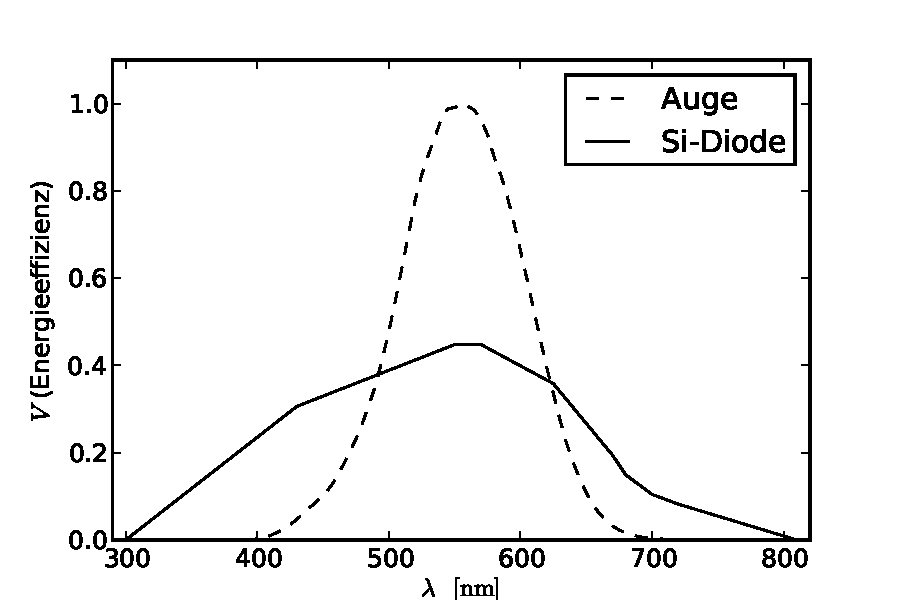
\includegraphics[width=0.75\textwidth]{images/lichteffizienz_silizium_auge.pdf}
\end{center}
\vspace{-1.5\baselineskip}
\caption{Energieeffizienz des menschlichen Auges und einer Si-Photodiode in Abhängigkeit von der Wellenlänge. Die Ordinate ist nicht auf Einheiten normiert.}
\label{lichteffizienz_auge}
\end{figure}
Um tatsächlich Lux zu messen, müsste der Sensor in etwa eine wellenlängenabhängige Empfindlichkeit wie in die des Auges\footnote{\url{http://www.cvrl.org}} aufweisen. Siliziumdioden, wie die im Sensor verbaute haben aber durchaus verschiedene Wellenlängenabhängigkeiten. Die meisten der im Internet gefundenen Datenblätter zeigen eine höhere Effizienz bei großen Wellenlängen mit einem Maximum um $800\unit{nm}$ herum. Photodioden, die dem Auge mehr ähneln, scheinen aber zu existieren. In Frage kommt z.B. ein Spektrum wie das der Silizium Photodiode S1133 von Hamamatsu\footnote{\url{http://sales.hamamatsu.com/assets/pdf/parts_S/S1087_etc.pdf}}. Die Spektren sind in Abb. \ref{lichteffizienz_auge} gezeichnet.


\subsubsection{Wellenlängenempfindlichkeit der Grätzelzelle}
Nimmt man nun die Si-Diodenempfindlichkeitskurve als Schätzung für die Sensorempfindlichkeit $V$ her, so ergibt sich für die tatsächliche Helligkeit $\Phi$ einer LED:
\[
E_{\text{mess}}(\lambda) = \Phi(\lambda)\cdot V(\lambda)
\qquad\Rightarrow\qquad
\Phi(\lambda) = \frac{E_{\text{mess}}(\lambda)}{V(\lambda)}
\]
Die relative Farbempfindlichkeit ergibt sich nun einfach aus $U/\Phi$. Die so berechneten und auf 1 normierten Werte sind in Tabelle \ref{lambda_kurve} aufgelistet.
\begin{table}[ht]
\captionabove{Tatsächliche LED-Helligkeiten $\Phi$ und relative Effizienz der Photozelle}
\label{lambda_kurve}
\begin{center}\vspace{-\baselineskip}
\begin{tabular}{l|ccc}
\# &
$\lambda\; \unit{[nm]}$ &
$\Phi / \Phi_{\text{max}}$ &
$E/E_{\text{max}}$ \\
\hline
LED1	& 627	& 0.843	& 0.047 \\
LED2	& 617	& 0.734	& 0.067 \\
LED3	& 590	& 0.193	& 0.159 \\
LED5	& 505	& 0.711	& 0.588 \\
LED6	& 470	& 0.919	& 0.855 \\
LED7	& 455	& 1.000	& 1.000
\end{tabular}
\vspace{-\baselineskip}\end{center}
\end{table}
Die Energieeffizienz der Grätzelzelle lässt nun eine eindeutige Wellenlängenabhängigkeit erkennen, die für kleine Wellenlängen deutlich höher ist. Insgesamt waren nicht genügend verschiedene Spektralbereiche zur Messung vorhanden um Sprünge oder genauere Details erkennen zu können. Aber es kann leicht nachvollzogen werden, dass eine monotone Abhängigkeit vorhanden ist, und höherenergetische Photonen deutlich mehr zur Leistung beitragen.
\begin{figure}[ht]
\begin{center}
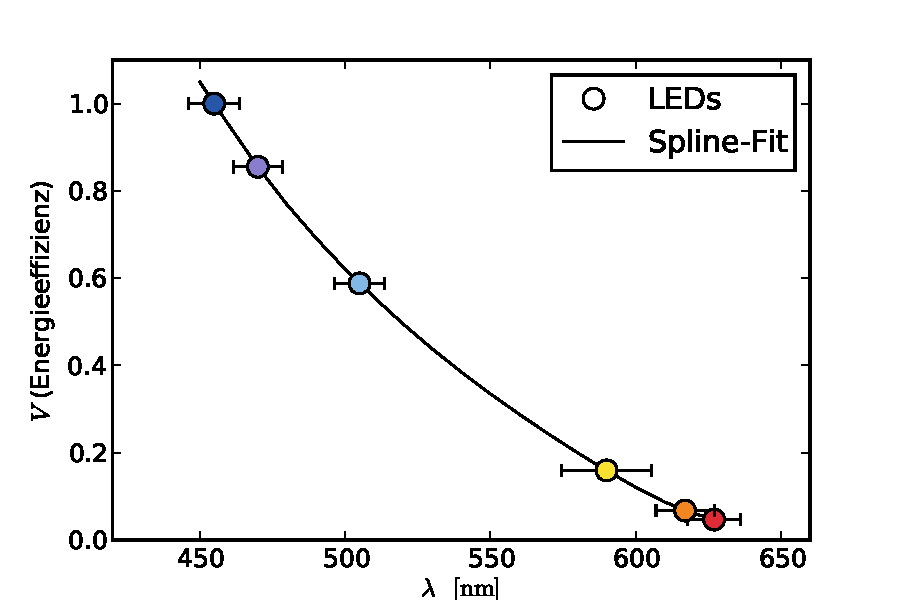
\includegraphics[width=1.0\textwidth]{images/graetzel_lambda_korrigiert.pdf}
\end{center}
\vspace{-1.5\baselineskip}
\caption{relative Energieeffizienz der Grätzelzelle in Abhängigkeit von der Wellenlänge. Jeder Datenpunkt wurde mit der Referenzmessung des Luxsensors und der Effizienzkurve für die Siliziumdiode kalibriert.}
\label{lambda_korrigiert}
\end{figure}

Die Unsicherheit der Werte in $y$-Richtung ist trotz aller Bemühungen relativ groß, aber nicht quantifizierbar, da sie direkt von der Diode des Cassy Luxsensors abhängt. Effektiv wird die Ergebniskurve direkt proportional mit der Detektorcharakteristik multipliziert. Wurde z.B. eine weniger augenähnliche Diode verbaut, die bei großen Wellenlängen empfindlicher ist, so würde sich auch unsere Kurve dort nach oben verschieben und nicht mehr ganz so steil sein. Der Effekt wäre aber höchstwahrscheinlich nicht groß genug um den Trend umzukehren, da dieser ziemlich eindeutig hervortritt. Die Erkenntnis bleibt: Die Grätzelzelle liefert bei höherenergetischen Photonen deutlich mehr Leistung.


\section{Fazit}
%%% zusammen
Dank an Dr. Vito Sgobba, etc.
\end{document}

